\documentclass[a4paper,
fontsize=11pt,
%headings=small,
oneside,
numbers=noperiodatend,
parskip=half-,
bibliography=totoc,
final
]{scrartcl}

\usepackage[babel]{csquotes}
\usepackage{synttree}
\usepackage{graphicx}
\setkeys{Gin}{width=.4\textwidth} %default pics size

\graphicspath{{./plots/}}
\usepackage[ngerman]{babel}
\usepackage[T1]{fontenc}
%\usepackage{amsmath}
\usepackage[utf8]{inputenc} % utf8x is deprecated and clashes with modern packages
\usepackage [hyphens]{url}
\usepackage{booktabs}
\usepackage{array}      % needed for >{...} column modifiers
\usepackage{ragged2e}   % \RaggedRight with hyphenation inside table cells
\usepackage{needspace}  % keep code blocks from splitting across pages

\usepackage[left=2.4cm,right=2.4cm,top=2.3cm,bottom=2cm,includeheadfoot]{geometry}
\usepackage[labelformat=empty]{caption} % option 'labelformat=empty]' to surpress adding "Abbildung 1:" or "Figure 1" before each caption / use parameter '\captionsetup{labelformat=empty}' instead to change this for just one caption
\usepackage{eurosym}
\usepackage{multirow}
\usepackage[ngerman]{varioref}
\setcapindent{1em}
\renewcommand{\labelitemi}{--}
\usepackage{paralist}
\usepackage{pdfpages}
\usepackage{float}
\usepackage{acronym}
\usepackage{longtable,lscape}
\usepackage{mathpazo}
\usepackage[normalem]{ulem} %emphasize weiterhin kursiv
\usepackage[flushmargin,ragged]{footmisc} % left align footnote
\usepackage{ccicons} 
\setcapindent{0pt} % no indentation in captions
\usepackage{xurl} % Breaks URLs

% float placement: let big tables/figures share a page with text
\renewcommand{\topfraction}{0.9}
\renewcommand{\bottomfraction}{0.8}
\renewcommand{\textfraction}{0.07}
\renewcommand{\floatpagefraction}{0.8}
\setcounter{topnumber}{2}
\setcounter{bottomnumber}{2}
\setcounter{totalnumber}{4}

%%%% fancy LIBREAS URL color 
\usepackage{xcolor}
\definecolor{libreas}{RGB}{112,0,0}

\usepackage{listings}

%%%% SPARQL syntax highlighting %%%%
\definecolor{sparqlkw}{RGB}{112,0,0}      % keywords (LIBREAS red)
\definecolor{sparqlprefix}{RGB}{0,90,140} % wdt:, wd:, bd:, wikibase:
\definecolor{sparqlvar}{RGB}{140,70,0}    % ?variables
\definecolor{sparqlstr}{RGB}{20,110,60}   % "strings"
\definecolor{sparqlbg}{RGB}{248,246,244}  % code background
\definecolor{sparqlrule}{RGB}{200,192,186}

\lstdefinelanguage{SPARQL}{
  % SPARQL keywords
  morekeywords={SELECT,WHERE,SERVICE,GROUP,BY,ORDER,DESC,ASC,COUNT,AS,
    FILTER,OPTIONAL,DISTINCT,LIMIT,OFFSET,PREFIX,BIND,VALUES,UNION,
    MINUS,HAVING,CONSTRUCT,ASK,DESCRIBE,REDUCED,STR,LANG,SAMPLE},
  % Wikidata / RDF namespace prefixes (no ':' in alsoletter, so these
  % are separate tokens and get highlighted)
  morekeywords=[2]{wdt,wd,bd,wikibase,rdfs,rdf,schema,p,ps,pq,psv,xsd,owl},
  sensitive=false,
  morecomment=[l]{\#},
  morestring=[b]",
  alsoletter={?_},
}

\lstdefinestyle{sparqlstyle}{
  language=SPARQL,
  basicstyle=\footnotesize\ttfamily,
  keywordstyle=\bfseries\color{sparqlkw},
  stringstyle=\color{sparqlstr},
  commentstyle=\itshape\color{gray},
  backgroundcolor=\color{sparqlbg},
  frame=single,
  rulecolor=\color{sparqlrule},
  framesep=6pt,
  xleftmargin=6pt,
  xrightmargin=6pt,
  breaklines=true,
  breakatwhitespace=true,
  breakindent=2em,
  postbreak=\mbox{\textcolor{sparqlrule}{$\hookrightarrow$}\space},
  columns=fullflexible,
  keepspaces=true,
  showstringspaces=false,
  tabsize=2,
  aboveskip=1.2\baselineskip,
  belowskip=1.2\baselineskip,
  % colour ?variables and prefix:names
  emph={[2]wdt,wd,bd,wikibase,rdfs,schema,p,ps,pq},
  emphstyle={[2]\color{sparqlprefix}},
}
\lstset{style=sparqlstyle}

\urlstyle{same}  % don't use monospace font for urls

\usepackage[fleqn]{amsmath}

%adjust fontsize for part

\usepackage{sectsty}
\partfont{\large}

%Das BibTeX-Zeichen mit \BibTeX setzen:
\def\symbol#1{\char #1\relax}
\def\bsl{{\tt\symbol{'134}}}
\def\BibTeX{{\rm B\kern-.05em{\sc i\kern-.025em b}\kern-.08em
    T\kern-.1667em\lower.7ex\hbox{E}\kern-.125emX}}

\usepackage{fancyhdr}
\fancyhf{}
\pagestyle{fancyplain}
\fancyhead[R]{\thepage}

% make sure bookmarks are created eventough sections are not numbered!
% uncommend if sections are numbered (bookmarks created by default)
\makeatletter
\renewcommand\@seccntformat[1]{}
\makeatother

% typo setup
\clubpenalty = 10000
\widowpenalty = 10000
\displaywidowpenalty = 10000

% --- prevent overfull lines (e.g. "...stellen diesen Dienst" in the abstract) ---
\usepackage{microtype}          % protrusion + font expansion, removes most overfull boxes
\emergencystretch=2em           % last-resort stretch instead of running into the margin
\tolerance=1200
\hbadness=1200                  % don't report merely loose lines
\setlength{\headheight}{26pt}   % silence the fancyhdr \headheight warning
\setlength{\headsep}{18pt}

% hyperref must be loaded BEFORE hyperxmp.
% breakurl is a dvips-only package and is redundant here (xurl is loaded above).
\usepackage[colorlinks, linkcolor=black,citecolor=black, urlcolor=libreas,
breaklinks= true,bookmarks=true,bookmarksopen=true]{hyperref}
\usepackage{hyperxmp}

%meta
%meta

\fancyhead[L]{Redaktion LIBREAS\\ %author
LIBREAS. Library Ideas, 48 (2026). % journal, issue, volume.
\href{https://doi.org/10.18452/}{\color{black}https://doi.org/10.18452/}
{}} % doi 
\fancyhead[R]{\thepage} %page number
\fancyfoot[L] {\ccLogo \ccAttribution\ \href{https://creativecommons.org/licenses/by/4.0/}{\color{black}Creative Commons BY 4.0}}  %licence
\fancyfoot[R] {ISSN: 1860-7950}

\title{\LARGE{Mehr Edits wagen? Virtuelle Ausstellungen erschließen mit Wikidata und Commons \\ WikiKult-Netzwerk und Deutsche Digitale Bibliothek kooperieren, um Metadaten zu pflegen}}% title
\author{Jens Bemme \& Alexander Winkler} % author

\setcounter{page}{1}

\hypersetup{%
      pdftitle={Mehr Edits wagen? Virtuelle Ausstellungen erschließen mit Wikidata und Commons},
      pdfauthor={Jens Bemme, Alexander Winkler},
      pdfsubject={LIBREAS. Library Ideas, 48 (2026)},
      pdfkeywords={Wikidata, Aktivismus, Metadaten, GLAM},
      pdflicenseurl={https://creativecommons.org/licenses/by/4.0/},
      pdfcopyright={CC BY 4.0 International},
      pdfcontacturl={http://libreas.eu},
      pdfurl={https://doi.org/10.18452/37905},
      pdfdoi={10.18452/37905},
      pdflang={de},
      pdfmetalang={de}
     }



\date{}
\begin{document}

\maketitle
\thispagestyle{fancyplain} 

%abstracts
\begin{abstract}
\noindent
\textbf{Zusammenfassung}: Was ist Metadatenaktivismus? Dieser Beitrag
skizziert Erschließungsarbeit, Motivation, Prinzipien und Perspektiven
für die Erschließung von virtuellen Ausstellungen, die seit 2019 mit
`DDBstudio', dem Ausstellungsservice der Deutschen Digitalen Bibliothek
(DDB) entstehen. Mittelkürzungen stellen diesen Dienst der DDB in Frage.
Ausgehend vom Netzwerk `WikiKult -- Offene Kulturdaten', einem freien
Zusammenschluss von Expert:innen aus dem Kulturerbesektor, werden
Ausstellungen der DDB seit Februar 2026 in Wikidata und in
Bibliothekssystemen erschlossen. Angesichts der wachsenden Kooperation
formulieren die Autoren nicht zuletzt das Ziel, dass Bibliotheken,
Archive und andere Kulturinstitutionen, insbesondere die Deutsche
Digitale Bibliothek und die Wikimedia-Bewegung, anhand und für
wirkungsvolle Projekte öfter zusammenarbeiten -- zum Beispiel für neue
virtuelle Ausstellungen über 2026 hinaus.

\noindent
\textbf{Abstract}: What is metadata activism? This article outlines the
work of cataloging, the motivation, principles, as well as perspectives
for cataloging virtual exhibitions created since 2019 with DDBstudio, an
exhibition service of the German Digital Library (DDB). Budget cuts are
jeopardizing this DDB service. Based on the `WikiKult -- Open Cultural
Data' network, an independent association of experts from the cultural
heritage sector, DDB exhibitions have been cataloged in Wikidata and
union catalogues since February 2026. In light of this growing
cooperation, the authors express the goal that libraries, archives,
other cultural institutions, like the DDB and the Wikimedia movement,
collaborate more frequently.
\end{abstract}

%body
\hypertarget{einfach-neue-ausstellungen-machen}{%
\section{Einfach neue Ausstellungen
machen?}\label{einfach-neue-ausstellungen-machen}}

Im Oktober 2019 startete die Deutsche Digitale Bibliothek
(DDB),\footnote{\url{https://www.deutsche-digitale-bibliothek.de}} das
zentrale Aggregationsorgan für digitalisiertes Kulturerbe in Deutschland
mit derzeit über 65 Millionen verzeichneten Objekten,
DDBstudio.\footnote{Vgl. die Pressemitteilung vom 8.10.2019:
  \url{https://www.deutsche-digitale-bibliothek.de/content/blog/ddbstudio-mit-virtuellen-ausstellungen-geschichten-erzaehlen-neuer-service-der-deutschen-digitalen-bibliothek/}}
DDBstudio ist ein Service, mit dem Kulturerbeinstitutionen gebührenfrei
und niedrigschwellig ansprechende virtuelle Ausstellungen erstellen und
publizieren können, ohne auf die kommerziellen und datenhungrigen
Alternativen US-amerikanischer Konzerne zurückgreifen zu müssen. Mit
virtuellen Ausstellungen können Objekte, die in der DDB oder anderswo
veröffentlicht sind, in narrativen, thematischen Zusammenhängen
präsentiert werden: in Geschichten, mit Hintergründen und Verknüpfungen
für digitale \enquote*{Geschichten}, und damit in einer Weise, wie dies
in der objektfokussierten Standarddarstellung der DDB nicht möglich ist.
Damit ist DDBstudio ein wertvolles Instrument der Vermittlung, das von
den Kulturerbeeinrichtungen rege genutzt wird. Seit Ende 2019 sind 278
virtuelle Ausstellungen entstanden und einige mehr sind in
Vorbereitung.\footnote{Für einen Überblick vgl.
  \url{https://www.deutsche-digitale-bibliothek.de/content/virtuelle-ausstellungen}}

Im Februar 2026 machte die Nachricht die Runde, dass die DDB durch
Mittelkürzungen gezwungen sei DDBstudio einzustellen.\footnote{Deutsche
  Digitale Bibliothek: Newsletter, Virtuelle Austellungen, Februar 2026,
  \url{https://www.deutsche-digitale-bibliothek.de/content/newsletter/newsletter-virtuelle-ausstellungen-februar-2026}}
Die für die Betreuung des Angebots nötigen Personalressourcen könnten
nicht mehr finanziert werden. Unveröffentlichte Ausstellungen werden
noch ergänzt, ältere bleiben online -- vorerst zumindest.

Die finanziellen Einschnitte trafen die DDB hart -- und mit ihr die
digitalisierenden Kulturerbeinstitutionen ebenso wie die Bürger:innen,
die digitales Kulturerbe rezipieren und nutzen. Mit der DDB fehlt in
diesem Jahr auf der Leipziger Buchmesse und bei der BiblioCon, zwei
zentralen Veranstaltungen des deutschen Buch- und Bibliothekswesens,
eine wichtige Stimme der kulturellen Daseinsvorsorge im digitalen Raum.

Beim monatlichen Jour Flexe des Netzwerks \enquote*{WikiKult -- Offene
Kulturdaten}, dem freien Zusammenschluss von Expert:innen in
Kulturerbeeinrichtungen, waren diese Kürzungen im Februar 2026
Gesprächsthema.\footnote{\url{https://meta.wikimedia.org/wiki/WikiKult_-_Offene_Kulturdaten}}
Die erste Idee: Wie können wir mit Wikimedia Commons, Wikidata oder
Wikiversity -- allgemein: mit Werkzeugen und Ressourcen des
Wikiversums\footnote{Zum Begriff \enquote*{Wikiversum}, mit dem
  Wikipedia und ihre Schwesterprojekte wie z.\,B. Wikidata, Wikimedia
  Commons und Wikisource gemeint sind, vgl.
  \url{https://de.wikipedia.org/wiki/Wikiversum}.} -- neue virtuelle
Ausstellungen ermöglichen, wenn DDBstudio dafür nicht mehr zur Verfügung
stehen sollte? Der daraus entstehende Impuls:
Metadatenaktivismus.\footnote{Wikidata: Metadatenaktivismus
  (\href{http://www.wikidata.org/entity/Q138306679}{Q138306679})} Wir
erschließen einfach die bisher veröffentlichten DDB-Ausstellungen mit
Wikidata selbst, um die Ausstellungsdaten beziehungsweise deren
Metadaten \enquote*{linked open} zu sichern.\footnote{Vgl.
  \url{https://osl.hypotheses.org/23842}}

\begin{figure}
\centering
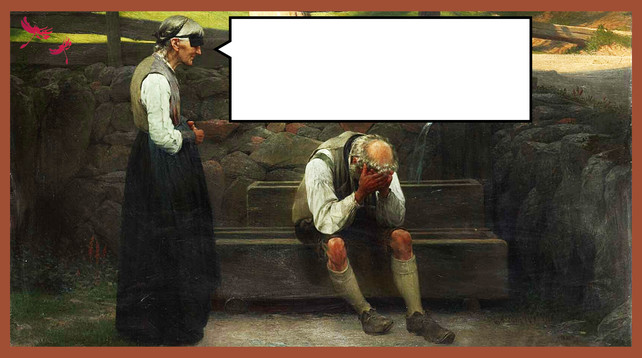
\includegraphics{Trostworte_DDB.jpg}
\caption{Social Media-Bildvorlage der DDB: Gemälde von Konrad Dielitz,
\href{https://commons.wikimedia.org/wiki/File:Trostworte_DDB.jpg}{Trostworte}
(\href{http://www.wikidata.org/entity/Q50120344}{Q50120344}) und eine
leere Sprechblase.
(\href{https://creativecommons.org/publicdomain/zero/1.0/deed.en}{CC0})}
\end{figure}

Mittlerweile wurde zwar die Wiederaufnahme des DDBstudio ab September
2026 bekannt gegeben, allerdings mit eingeschränktem Service und nur
noch für aktive Datenpartner der DDB.\footnote{Vgl.
  \url{https://www.deutsche-digitale-bibliothek.de/content/blog/virtuelle-ausstellungen-bleiben-ein-angebot-der-deutschen-digitalen-bibliothek}}

\hypertarget{ad-hoc-katalogisierung-call-for-edits}{%
\subsection{Ad-hoc-Katalogisierung -- Call for
Edits}\label{ad-hoc-katalogisierung-call-for-edits}}

WikiKult hat bereits im Mai 2025, also lange vor Ankündigung der
Mittelkürzung, ein erstes Set frei zugänglicher, semi-strukturierter
Metadaten der DDB-Ausstellungen extrahiert, aufbereitet und in Wikidata
veröffentlicht, weil die DDB als ein wichtiger Baustein der deutschen
Open-GLAM-Infrastruktur größere Sichtbarkeit im Wikiversum und im
Linked-Open-Datenraum verdient. Die virtuellen Ausstellungen sollten so
als eigenständige Produkte für die Rezeption und Vermittlung von
Kulturerbe dokumentiert werden. Eine weitere Motivation hinter dieser
Metadatenarbeit: Die selbstgestellte Aufgabe, semistrukturiert
vorliegende Daten für die Linked-Open-Welt aufzubereiten, ist anregend
und in gewisser Weise auch sinnstiftend. Informationen werden dadurch
besser auffindbar, leichter zugänglich, interoperabler und besser
nutzbar, kurz: FAIR. Insbesondere die Verwendung von Wikidata kann ein
integraler Bestandteil des Strebens nach FAIR(er)en Daten sein. Hinter
dem schon bemühten Akronym
\href{https://www.go-fair.org/fair-principles/a2-metadata-accessible-even-data-no-longer-available/}{FAIR}
stehen zentrale Qualitätskriterien für gut nutzbare Forschungsdaten.
Daten sollen \emph{\underline{f}indable}, \emph{\underline{a}ccessible},
\emph{\underline{i}nteroperable} und \emph{\underline{r}eusable} sein.

Die Ausstellungen der DDB verfügen originär über keine expliziten
Metadaten, zum Beispiel im Sinne eines Katalogisats. Sie stehen als
Webangebote für sich, sind auf einer Übersichtsseite der DDB lediglich
mit ihrem Titel aufgelistet und die einzelnen Ausstellungen verfügen
über nur schwach strukturierte Angaben, wie zum Beispiel Urheber:innen
oder Veröffentlichungsdatum. Die FAIR-Prinzipien erfordern jedoch
explizite, maschinenlesbare und nötigenfalls über die Lebensdauer des
Objekts hinaus persistente Metadaten. Eine Erschließung in Wikidata
erzeugt zusätzlich Metadaten, die diese Anforderungen erfüllen.

Aufbauend auf diesem schon gelegten Fundament haben wir nach der
bitteren Nachricht im Februar 2026 beschlossen, weitere Informationen
über die virtuellen Ausstellungen zusammenzutragen und in Wikidata zu
ergänzen, insbesondere folgende Angaben:

% helper: a Wikidata link that is allowed to break and never overflows
\newcommand{\wdlink}[2]{\href{https://www.wikidata.org/wiki/#1}{(#2)}}

\begin{table}[tbp]
\footnotesize
\setlength{\tabcolsep}{5pt}
\renewcommand{\arraystretch}{1.25}
\caption{Tabelle 1: Zusätzliche Informationen über die virtuellen
Ausstellungen in Wikidata inklusive Beispielen}
\begin{tabular}{@{}
  >{\RaggedRight}p{0.27\textwidth}
  >{\RaggedRight}p{0.18\textwidth}
  >{\RaggedRight\arraybackslash}p{0.47\textwidth}@{}}
\toprule
\textbf{Aussage} & \textbf{Wikidata-Property} & \textbf{Beispiel} \\
\midrule

zentrale Themen / Schlagworte & P921 & --- \\

Datum der Veröffentlichung & P577 & --- \\

Publizierende Institution & P123 &
  \emph{Als Weihnachten ins Wasser fiel. Remshochwasser 1919}\newline
  \wdlink{Q134475380\#P123}{Q134475380\#P123} \\

Bilder, die bereits in Wikimedia Commons vorliegen & P18 &
  \emph{Himmelswege. Formen spätmittelalterlicher Laienfrömmigkeit im
  mitteldeutschen Raum}\newline
  \wdlink{Q134475329\#P18}{Q134475329\#P18} \\

Sprachvarianten wie Englisch und Albanisch &
  Sprache (P407)\newline Titel (P1476)\newline offizielle Webseite (P856) &
  \emph{Spotlight on the Object \textbar{} PERSON, PLACE or THING}\newline
  \wdlink{Q134475369}{Q134475369}\newline
  \emph{Tiranë, Korrik 1990 -- Tirana, Juli 1990}\newline
  \emph{Arratisje në Ambasadën Gjermane -- Flucht in die Deutsche
  Botschaft}\newline
  \wdlink{Q134475231\#P407}{Q134475231\#P407} \\

URL des Archivs (Internet Archive) & P1065 &
  \emph{Zitrusmanie. Goldene Früchte in fürstlichen Gärten},
  Qualifier (P1065) in\newline
  \wdlink{Q134475228\#P856}{Q134475228\#P856} \\

Wikimedia Commons-Kategorie für Ausstellungsbilder & P373 &
  \emph{Category:DDBstudio Gemeinsam für Freies Wissen}\newline
  \wdlink{Q134475374\#P373}{Q134475374\#P373} \\

reziproke Aussage \enquote*{beschrieben in} für QID zentraler Themen & P1343 &
  \emph{Pädagogische Lesungen}\newline
  \wdlink{Q102227101\#P1343}{Q102227101\#P1343} \\

K10plus PPN ID & P6721 &
  \emph{Die kontaminierte Bibliothek. Mikroben in der Buchkultur}\newline
  \wdlink{Q134475219\#P6721}{Q134475219\#P6721} \\

zitiert & P2860 &
  \emph{Ankunft auf Zeit. Die Cottbuser Kriegsgefangenenlager von 1914
  bis 1924}\newline
  \wdlink{Q134475352\#P2860}{Q134475352\#P2860} \\

Katalog (Regionalbibliografie) & P972 &
  \emph{Zum Shopping in die DDR. Die DDR-Einkäufe des West-Berliner
  Museums für Verkehr und Technik}\newline
  \wdlink{Q134475238\#P972}{Q134475238\#P972} \\

\bottomrule
\end{tabular}
\end{table}

\hypertarget{wikimedia-commons}{%
\section{Wikimedia Commons}\label{wikimedia-commons}}

Einige virtuelle Ausstellungen enthalten Bilder mit Quellenangabe und
Link zur entsprechenden Ressource in Wikimedia Commons. Auch Bilder ohne
Verweis auf Wikimedia Commons sind dort trotzdem zu finden. All diese
Illustrationen können in neu erstellten Ausstellungskategorien gebündelt
werden, die als Unterkategorien in der Commons-Kategorie der DDB
verlinkt sind.\footnote{\url{https://commons.wikimedia.org/wiki/Category:Deutsche_Digitale_Bibliothek}}
Selbstverständlich könnten nun in spezifische Ausstellungskategorien in
Wikimedia Commons weitere offen lizenzierte Ausstellungsbilder geladen
und somit ergänzt werden. Dann stehen sie im Wikiversum für Einbettungen
in Wikipedia und Wikiversity oder im Idealfall für Bearbeitungen und
auch für die allgemeine Nachnutzung zur Verfügung. Wikidata-Infoboxen
für solche Kategorien verknüpfen und zeigen Metadaten der zugehörigen
Datenobjekte in Wikidata für jede Ausstellung. Durch Kategorisierungen
am unteren Bereich der Commons-Seiten können die Ausstellungskategorien
den beteiligten Institutionen oder Personen und Themen zugeordnet
werden, deren Commons-Kategorien ihrerseits Inhalte und gegebenenfalls
Unterthemen bündeln, um dieses objektbasierte Wissen zu strukturieren.

\begin{figure}
\centering
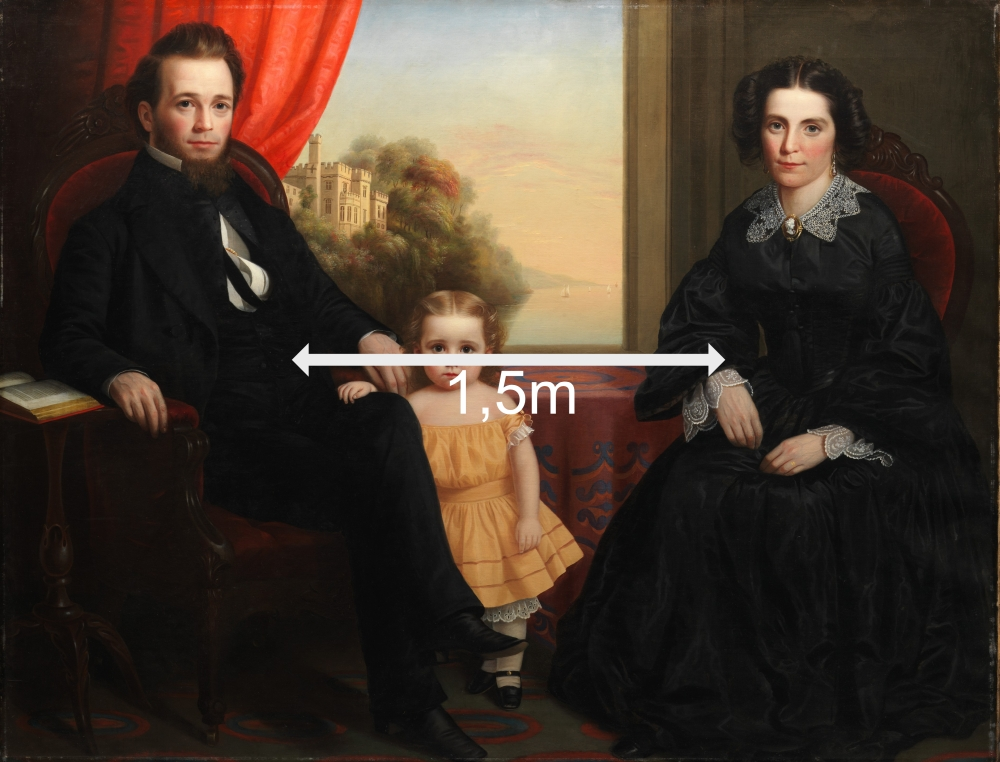
\includegraphics{A_Family_Group_DDB_2020.jpg}
\caption{Illustration: Collage auf Basis von Anonymous: A Family Group,
in der Virtuelle Ausstellung 'Rühr mich nicht an! Zur Kulturgeschichte
des Social Distancing, 2020
\url{https://commons.wikimedia.org/wiki/File:A_Family_Group_DDB_2020.jpg}
(\href{https://creativecommons.org/publicdomain/zero/1.0/deed.en}{CC0})}
\end{figure}

Die Ausstellungserschließung in Wikidata ist längst nicht abgeschlossen,
weitere Präsentationen sollen folgen. Wir haben eine Dokumentation
angelegt, mit der Ausstellungsmacher:innen und auch die
DDB-Geschäftsstelle selbst im Zuge von Neuveröffentlichungen Metadaten
mit Wikidata dokumentieren und vernetzen könnten.\footnote{\url{https://meta.wikimedia.org/wiki/WikiKult_-_Offene_Kulturdaten/Virtuelle_Ausstellungen}}
Die Doku kann von allen einfach ergänzt werden, getreu dem Motto
\enquote{it is open, it's a wiki}. Dort gesammelte Links, Hinweise und
Fragen können als Anregungen für ähnlich gelagerte Vorhaben dienen und
als digitale Spuren solcher verknüpften
Erschließungsgeschichten.\footnote{Vgl.
  \url{https://osl.hypotheses.org/20726} und
  \url{https://osl.hypotheses.org/21392}}

Deutlich wird das Potential für Kontextualisierungen der
Ausstellungsinhalte durch Commons-Kategorien am Beispiel der Ausstellung
\enquote*{Albrecht Dürer -- 500 Jahre Meisterstiche}. Da für Dürers
Stiche teils mehrere digitalisierte Versionen, Bildausschnitte und
Varianten existieren, sind diese in bildspezifischen Commons-Kategorien
gebündelt und mit Wikidata verknüpft. Die Ausstellungskategorie
\href{https://commons.wikimedia.org/wiki/Category:DDBstudio_Albrecht_D\%C3\%BCrer_\%E2\%80\%93_500_Jahre_Meisterstiche}{Category:DDBstudio
Albrecht Dürer -- 500 Jahre Meisterstiche} bündelt die gezeigten Stiche,
so dass Besucher:innen diese erweiterten Ausstellungsräume zusätzlich in
Wikimedia Commons erkunden können.

\hypertarget{beifang-datenpflege-ii.-ordnung}{%
\section{Beifang: Datenpflege II.
Ordnung}\label{beifang-datenpflege-ii.-ordnung}}

Als Beifang kann die indirekte Datenpflege an \enquote*{benachbarten}
Themen und Datenobjekten bezeichnet werden. Ausstellungsmacher:innen in
Wikidata\footnote{Jens Bemme, Martin Munke: Call for Edits Nearby: Open
  Archives Metadata from Saxony. \url{https://doi.org/10.5334/johd.430}}
-- Archiven, Bibliotheken, Vereine und andere Initiativen -- profitieren
zusätzlich, wenn wir ihre institutionellen Metadaten in Wikidata
nebenbei anreichern und verknüpfen. Bei der Formal- und Sacherschließung
von Ausstellungen und anderen Werken in Wikidata greifen wir meist auf
bereits bestehende Datenobjekte zurück, ergänzen und verbessern diese,
wenn sie noch leer, ohne Aussagen oder fehlerhaft sind -- und wir
schaffen neue Datenobjekte für die Themen und Gegenstände der virtuellen
Ausstellungen, um sie beispielsweise mit Normdaten der GND und VIAF zu
verknüpfen. Für die virtuellen Ausstellungen sind das beispielhaft die
neuen Wikidata-Items für die Arbeitsgruppe Kritische Geographien
globaler Ungleichheiten
(\href{http://www.wikidata.org/entity/Q138685193}{Q138685193}) in
Hamburg oder die Arbeitsstelle Pädagogische Lesungen
(\href{http://www.wikidata.org/entity/Q138758452}{Q138758452}) in
Rostock. Verknüpft sind diese nun reziprok mit Datenobjekten der
DDB-Ausstellungen jeweils in der Aussage (P1343 -- \enquote{beschrieben
in}), also
\href{https://www.wikidata.org/wiki/Q138758452\#P1343}{(Q138758452\#P1343)},
beziehungsweise ermittelbar über die Wikidata-Spezialabfrage
\enquote*{What links here}, die einen gegebenenfalls verlinkten Kontext
für jedes Datenobjekt anzeigt.\footnote{Zum Beispiel
  \url{https://de.wikipedia.org/wiki/Hilfe:Links_auf_diese_Seite} für
  die deutsche Wikipedia} Datenpflege an bereits bestehenden Items
beispielsweise für zitierte Zeitungen, Zeitschriften und andere
Publikationen umfasst neben formalen Metadaten fehlende Verknüpfungen
mit der Zeitschriftendatenbank ZDB, PPN oder OCLC-Ids. Ein Beispiel
hierfür: Die Märkische Volksstimme (1890--1933)
(\href{http://www.wikidata.org/entity/Q107499030}{Q107499030}) wird in
der Ausstellung \enquote*{Ankunft auf Zeit. Die Cottbuser
Kriegsgefangenenlager von 1914 bis 1924} erwähnt:
(\href{https://www.wikidata.org/wiki/Q134475352\#P2860}{Q134475352\#P2860}).
Am 22. März 2026 war dieses Item noch fast leer.\footnote{Wikidata:
  \url{https://www.wikidata.org/w/index.php?title=Q107499030\&oldid=2474652992}.}
Datenpflege erhöht so die Aussagekraft von Wikidata sowohl direkt für
die Zeitung als auch indirekt für die verknüpfte Ausstellung;
verbesserte Datenqualität verringert Verwechslungsgefahr, in diesem Fall
mit der Märkischen Volksstimme
(\href{http://www.wikidata.org/entity/Q107499030}{Q1957451}), die erst
ab 1946 erschien.

\hypertarget{katalogisierung-im-verbund}{%
\section{Katalogisierung im
Verbund}\label{katalogisierung-im-verbund}}

Idealerweise werden Ausstellungen in und virtuelle Ausstellungen von
Archiven und Bibliotheken auch bibliografisch erschlossen, um deren
Existenz zu dokumentieren und Inhalte sowie verknüpfte Medien dauerhaft
für die Wissenschaft sichtbar und zugänglich zu machen, zum Beispiel in
Ausstellungskatalogen und auf Webseiten.\footnote{Vgl. etwa das
  bayerische Kulturportal Bavaricon, das an der BSB angesiedelt ist und
  Ausstellungen regelmäßig auch im Bibliothekskatalog erschließt, siehe
  etwa die Ausstellung \enquote*{Revolution und Räterepubliken in Bayern
  1918/19}
  (\url{https://www.bavarikon.de/object/bav:BSB-CMS-0000000000003602})
  mit dem Katalogisat
  \url{https://opacplus.bsb-muenchen.de/title/BV046755805}.} Die
virtuellen Ausstellungen der DDB waren bisher nicht in Verbundkatalogen
erschlossen.

Inzwischen wurden DDB-Ausstellungen, die Saxonica enthalten, in der
Sächsischen Bibliografie erfasst\footnote{K10Plus:
  \url{https://opac.k10plus.de/DB=2.299/PPNSET?PPN=735684553} sowie
  Sächsische Bibliografie im K10Plus:
  \url{https://swb.bsz-bw.de/DB=2.304/SET=3/TTL=1/FAM?PPN=735684553}}
und deren PPN mit den Wikidata-Items in (P6721) verknüpft. Mit
fortschreitender Erschließung in Wikidata beziehungsweise neu
veröffentlichten Ausstellungen wächst diese Liste möglicherweise noch.
Zu wünschen wäre außerdem, dass auch andere Landes- und
Regionalbibliotheken regional relevante Ausstellungen in ihren
Regionalbibliografien erschließen.

\begin{figure}
\centering
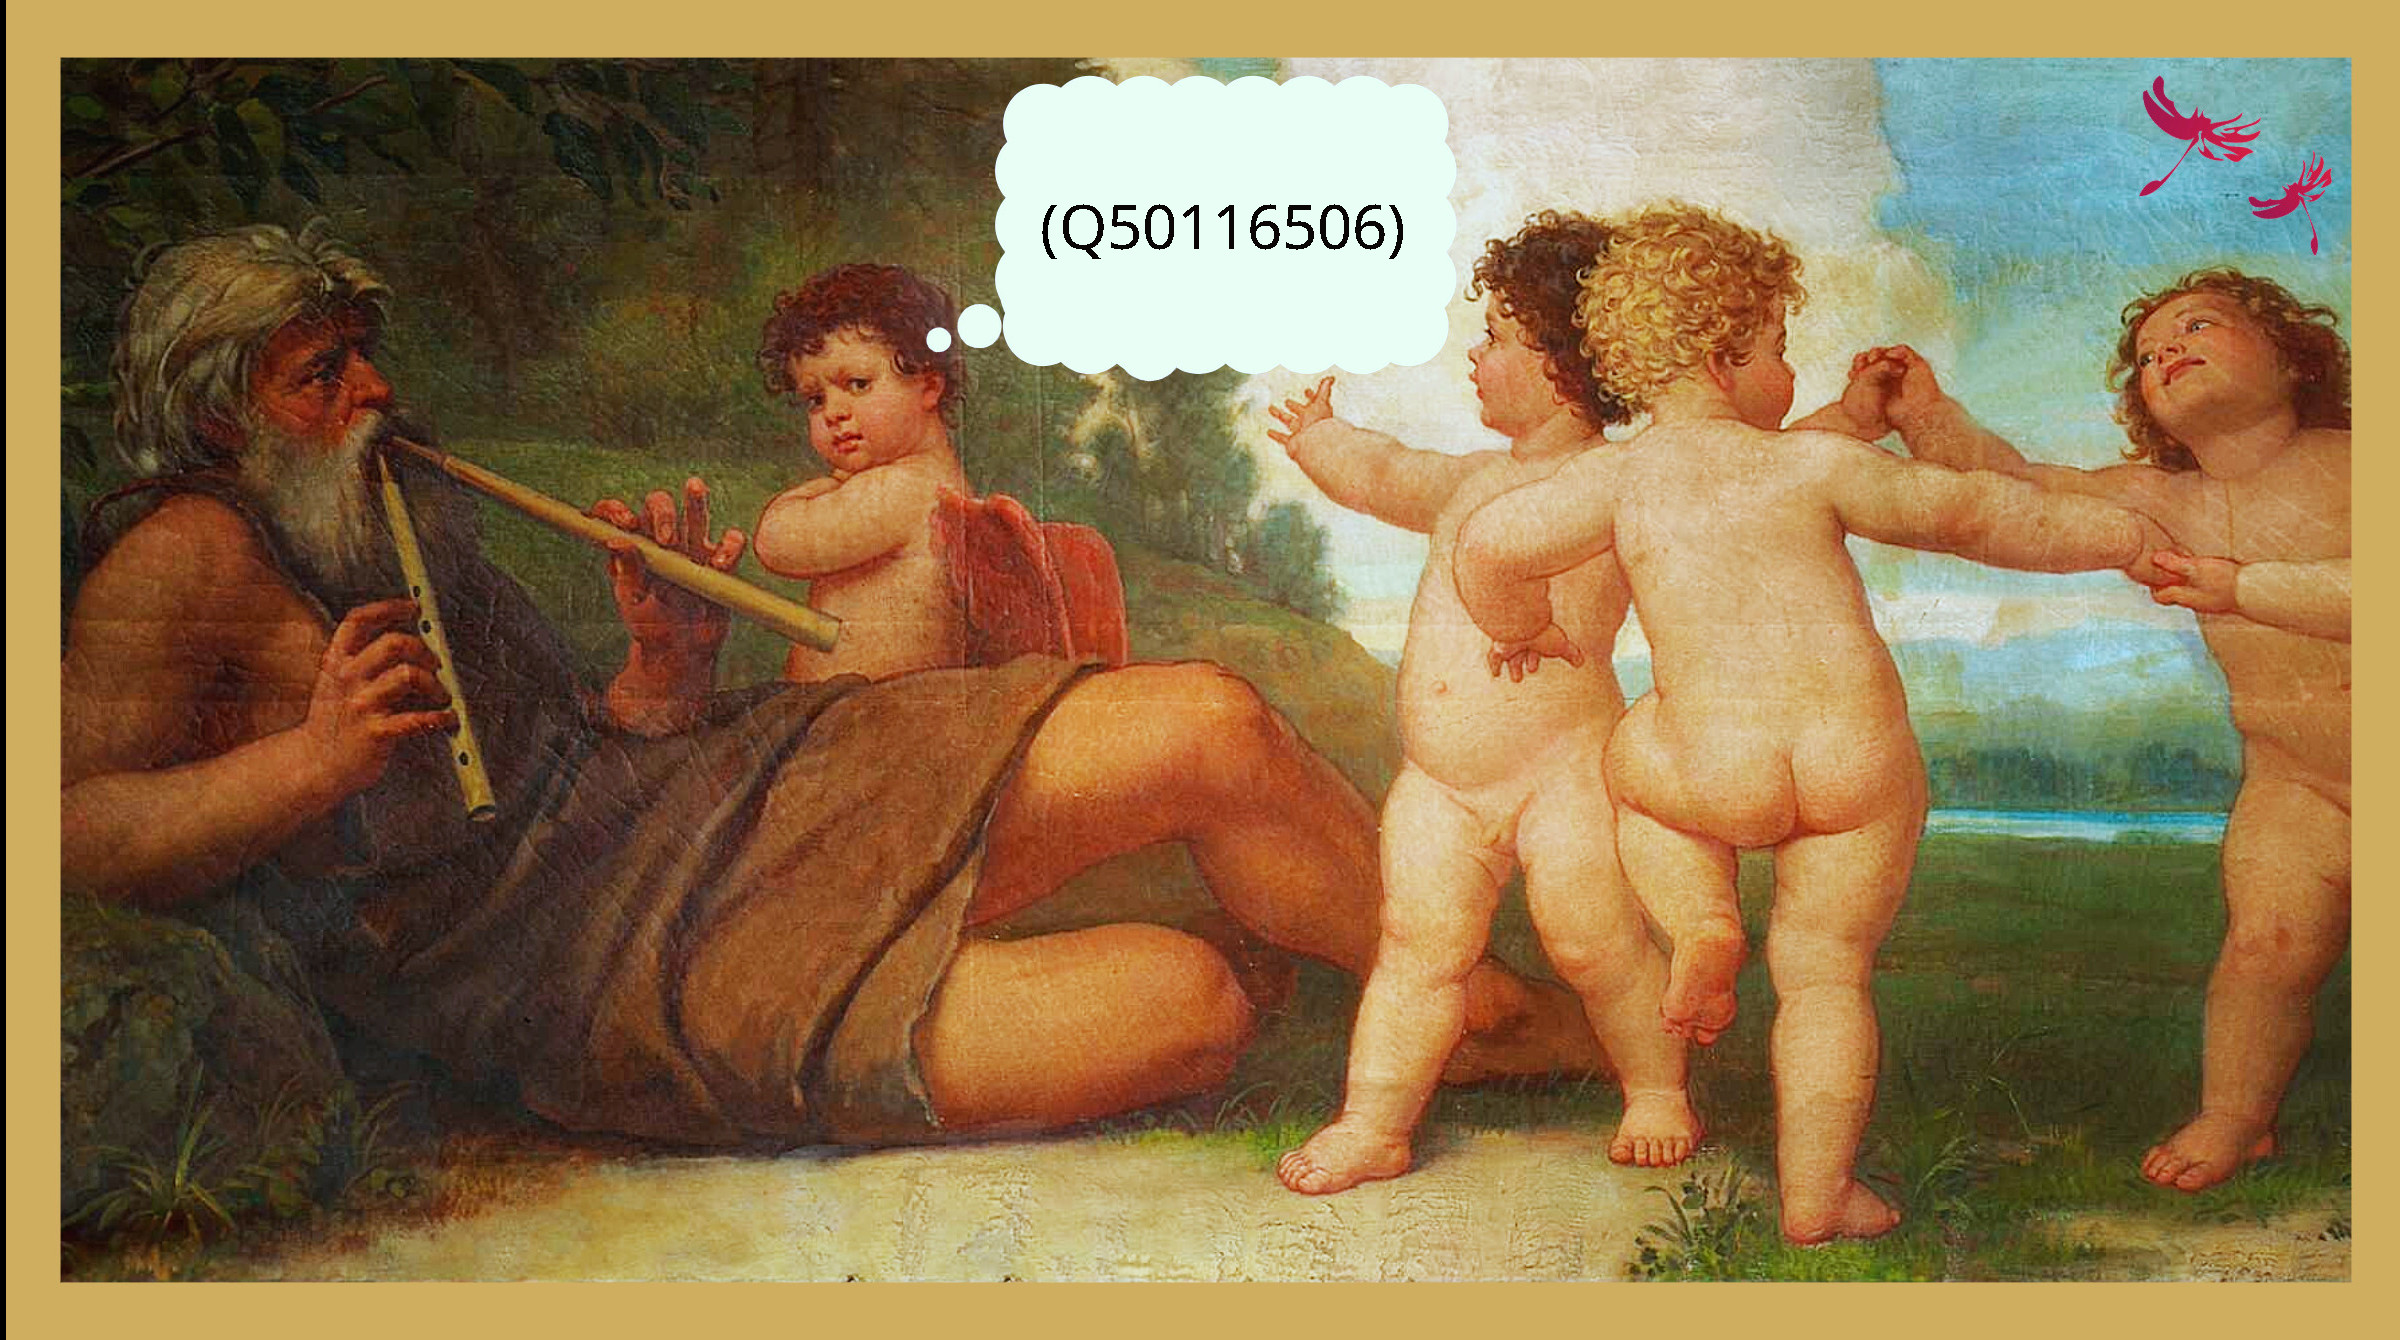
\includegraphics{Allegorie_auf_den_Fruehling_(Q50116506).jpg}
\caption{Illustration: Digitale Version Oskar Begas'
\href{https://www.deutsche-digitale-bibliothek.de/item/6T6E7TBIGN3ASDRZ4WYEXGXUTHMRN6PU}{Gemäldes}
'Allegorie auf den Frühling. Plafondbild aus dem Treppenhaus der
Berliner Villa Tiergartenstraße 27'
\url{https://commons.wikimedia.org/wiki/File:Allegorie_auf_den_Fr\%C3\%BChling_(Q50116506).jpg}
(\href{https://creativecommons.org/publicdomain/mark/1.0/deed.de}{Public
Domain})}
\end{figure}

\hypertarget{daten-strukturieren-datengrundlage-schaffen}{%
\section{Daten strukturieren -- Datengrundlage
schaffen}\label{daten-strukturieren-datengrundlage-schaffen}}

Die Informationen zu den Ausstellungen liegen auf der entsprechenden
Übersichtsseite\footnote{\url{https://www.deutsche-digitale-bibliothek.de/content/virtuelle-ausstellungen}}
schwach strukturiert als HTML-Code vor. Um vor einer tiefergehenden,
manuellen (und arbeitsintensiven) Erschließung zunächst eine kritische
Masse an Basisinformationen in Wikidata zu übernehmen, wurde die
Übersichtsseite -- wie oben beschrieben schon im Mai 2025 -- maschinell
ausgewertet, das heisst insbesondere die Titel und URLs der
Ausstellungen wurden mit einem Python-Script ausgelesen und in ein
strukturiertes Format (sprich: eine Tabelle) überführt. Dies war die
Datengrundlage für den Upload basaler Metadaten zu den Ausstellungen.
Der Upload erfolgte mit dem Quickstatements-Tool\footnote{\url{https://quickstatements.toolforge.org/\#/}},
das in tabellarischer Form vorliegende Informationen mit einem Minimum
an Befehlssyntax nach Wikidata lädt. In einem nächsten Schritt wurde im
Rahmen der systematischen Erschließung der Ausstellungen versucht, auf
den Seiten der einzelnen Ausstellungen weitere Informationen (wie zum
Beispiel das Publikationsdatum der Ausstellung) in eine strukturierte
Form zu bringen und ebenfalls über Quickstatements nach Wikidata zu
laden.

Der Vorteil dieses Vorgehens liegt in der Effizienz, da alle verfügbaren
Ausstellungen mit geringem Aufwand \emph{en bloc} in Wikidata
dokumentiert werden können, die aufwändigen manuellen Interventionen
also auf die Ergänzung von Informationen konzentriert werden konnten,
die nicht ohne Weiteres automatisiert zu erfassen sind.

\hypertarget{datenmodellierung}{%
\subsection{Datenmodellierung}\label{datenmodellierung}}

Wikidata zeichnet sich durch ein sehr flexibles Datenmodell aus. Es
stehen über 13.000 Properties zur Verfügung, mit denen Aussagen über
Wikidata-Items getroffen werden können.\footnote{Vgl.
  \url{https://www.wikidata.org/wiki/Wikidata:List_of_properties}} Die
Flexibilität bringt es mit sich, dass für die Beschreibung von
Wikidata-Objekten ein geeignetes Datenmodell ermittelt werden muss. Hier
bietet es sich an, Empfehlungen etablierter WikiProjekte zu
berücksichtigen. Für virtuelle Ausstellungen lohnt zum Beispiel ein
Blick auf das \emph{WikiProject Exhibitions}, das Properties aufführt,
mit denen sich typischerweise Ausstellungen gut beschreiben
lassen.\footnote{\url{https://www.wikidata.org/wiki/Wikidata:WikiProject_Exhibitions}}
Ergänzend und/oder alternativ lassen sich good practices auch aus
einschlägigen Wikidata-Items ableiten oder aber Tendenzen in der
Beschreibung über geeignete SPARQL-Queries ermitteln.

Für \enquote{Onlineausstellungen}
(\href{http://www.wikidata.org/entity/Q3062261}{Q3062261}) ergibt
beispielsweise folgender SPARQL-Query (\url{https://w.wiki/J7w5}) eine
Übersicht der verwendeten Properties:

\needspace{14\baselineskip}
\begin{lstlisting}
SELECT ?property ?propertyLabel (COUNT(?property) AS ?haeufigkeit)
WHERE {
  ?virtuelleAusstellung wdt:P31 wd:Q3062261 ;
                        ?p ?_ .
  ?property wikibase:directClaim ?p .
  SERVICE wikibase:label {
    bd:serviceParam wikibase:language "[AUTO_LANGUAGE],mul,en" .
  }
}
GROUP BY ?property ?propertyLabel
ORDER BY DESC(?haeufigkeit)
\end{lstlisting}

Die zwölf häufigsten Properties sind demnach:\footnote{Diese Statistik
  basiert auf aktuellen Daten und ist damit durch die bereits erfolgte
  Erschließung der DDB-Ausstellungen verzerrt.}

\begin{table}[H]
\centering
\small
\setlength{\tabcolsep}{8pt}
\renewcommand{\arraystretch}{1.2}
\caption{Tabelle 2: Überblick der häufigsten Properties für
\enquote{Onlineausstellungen} in Wikidata}
\begin{tabular}{@{}l >{\RaggedRight\arraybackslash}p{0.52\textwidth} r@{}}
\toprule
\textbf{Property} & \textbf{Label} & \textbf{Häufigkeit} \\
\midrule
P131  & liegt in der Verwaltungseinheit             & 10.672 \\
P31   & ist ein(e)                                  &  6.524 \\
P856  & offizielle Website                          &  6.228 \\
P17   & Staat                                       &  5.966 \\
P5008 & auf der Arbeitsliste des Wikimedia-Projektes &  5.876 \\
P664  & Veranstalter                                &  5.656 \\
P1476 & Titel                                       &  2.056 \\
P921  & zentrales Thema                             &    674 \\
P577  & Veröffentlichungsdatum                      &    255 \\
P407  & Sprache des Werks, Namens oder Begriffes    &    114 \\
P123  & Verlag                                      &    111 \\
P1344 & Teilnehmer an                               &     47 \\
\bottomrule
\end{tabular}
\end{table}

Diese Angaben bieten eine Orientierung, wie Onlineausstellungen in
Wikidata beschrieben werden können, sie müssen jedoch fallbezogen
angepasst werden. Für die Grunderschließung der virtuellen Ausstellungen
der DDB wurden regelmäßig Titel (P1476), die Deutsche Digitale
Bibliothek (\href{http://www.wikidata.org/entity/Q621630}{Q621630}) als
Veranstalter (P664), die publizierende Einrichtung als Verlag (P123) und
die Ausstellungs-URL als offizielle Website (P856) angegeben. Hinzu kam
schließlich noch das Veröffentlichungsdatum der Ausstellung (P577). Alle
Ausstellungen werden zudem als \enquote{Onlineausstellungen}
(\href{http://www.wikidata.org/entity/Q3062261}{Q3062261}) klassifiziert
(P31).

Folgender Query (\url{https://w.wiki/KFR2}) listet die bisher in
Wikidata nach beschriebenem Muster erschlossenen virtuellen
Ausstellungen der DDB auf:

\needspace{12\baselineskip}
\begin{lstlisting}
SELECT ?virtuelleAusstellung ?virtuelleAusstellungLabel
WHERE {
  ?virtuelleAusstellung wdt:P31 wd:Q3062261 ;
                        wdt:P664 wd:Q621630 .
  SERVICE wikibase:label {
    bd:serviceParam wikibase:language "[AUTO_LANGUAGE],mul,en" .
  }
}
\end{lstlisting}

\hypertarget{bemuxfchen-um-persistenz.-diy-webarchivierung-mit-der-wayback-machine}{%
\subsection{Bemühen um Persistenz. DIY-Webarchivierung mit der Wayback
Machine}\label{bemuxfchen-um-persistenz.-diy-webarchivierung-mit-der-wayback-machine}}

Die Mittelkürzungen bei der DDB mit der Streichung der virtuellen
Ausstellungen führen es deutlich vor Augen: Viele Inhalte und Angebote
sitzen auf einer prekären Infrastruktur auf, die nur so lange trägt, wie
sie finanziert wird. So scheint es nicht mehr ausgeschlossen, dass auch
die bestehenden, mühsam erstellten und wertvollen virtuellen
Ausstellungen der DDB irgendwann dem Rotstift zum Opfer fallen. Um dem
Risiko eines vollständigen Gedächtnisverlusts möglichst vorzubeugen,
müssen die Ausstellungen archiviert werden. Als Online-Publikationen
dürften die Ausstellungen zwar theoretisch in den Sammelauftrag der
Landesbibliotheken oder der Deutschen Nationalbibliothek fallen,
praktisch scheint eine Archivierung jedoch bis dato nicht zu erfolgen.

Als eine alternative Archivierungsmöglichkeit, die auch unabhängigen
Initiativen offensteht, bietet sich die WayBack-Machine des Internet
Archive an.\footnote{\url{https://web.archive.org/}}

Die in Wikidata nunmehr strukturiert vorliegenden Ausstellungs-URLs
wurden automatisiert im Internet-Archive gespeichert und die Archiv-URLs
über den Qualifier P1065 (URL des Archivs) zur Angabe der offiziellen
Website (P856) ergänzt. Somit ist die Ausstellung im Internet Archive
archiviert und der Nachweis über Wikidata dokumentiert. Sollte es also
dazu kommen, dass auch die bestehenden Ausstellungen offline gehen,
lassen sich über das Wikidata-Item nicht nur basale Metadaten über die
Ausstellung abrufen, sondern man gelangt über den Archivlink auch zur
archivierten Version der Ausstellung im Internet Archive.

\hypertarget{ausstellungen-einfach-machen}{%
\section{Ausstellungen einfach
machen}\label{ausstellungen-einfach-machen}}

\hypertarget{wissenskommunikation-linked-open}{%
\subsection{Wissenskommunikation linked
open}\label{wissenskommunikation-linked-open}}

Der Ansatz hinter den hier skizzierten offenen Arbeitsweisen mit
Wikidata und Links wurde an anderer Stelle bezeichnet als
\enquote*{Linked Open Storytelling} mit offenen Kulturdaten, mit deren
offenen Metadaten und mit Links von Projekten, Publikationen
beziehungsweise wie in diesem Fall mit virtuellen Ausstellungen und
ihren Metadaten.\footnote{Wikidata: Linked Open Storytelling,
  \url{https://www.wikidata.org/wiki/Q66631860\#P973}} Kollaborative
Erschließung und Archivierung der DDB-Ausstellungen wären ohne Social
Media -- namentlich ohne Tröts und Links im Fediverse -- wohl kaum
zustande gekommen. Der Impuls zur Erschließung erfolgte in einem
Mastodon-Post.\footnote{\url{https://openbiblio.social/@awinkler/116073539902876609}}
Der wurde dort von der regen Bibliotheks-Community aufgegriffen. Die
Arbeit an den Metadaten wird durch weitere Posts\footnote{\url{https://openbiblio.social/tags/ddbstudio}}
begleitet und ist in Blogposts\footnote{Jens Bemme (15. Februar 2026).
  DDB-Ausstellungen: Eröffnen, besuchen, \enquote*{putzen} -- Nutzen.
  Zeit für Metadatenaktivismus. \emph{SLUB Open Science Lab}. Abgerufen
  am 22. März 2026 von \url{https://doi.org/10.58079/15oza} sowie (23.
  März 2026). Ausstellungsdaten kuratieren für die Deutsche Digitale
  Bibliothek. \emph{SLUB Open Science Lab}. Abgerufen am 23. März 2026
  von \url{https://doi.org/10.58079/15s59}.} dokumentiert. Im Fediverse
wurde schließlich auch das Team der DDB-Geschäftsstelle auf die
Erschließungsaktivitäten aufmerksam, was zu einem Onlinetreffen und dann
zu engerem Austausch zwischen Wikikult-Mitgliedern und der DDB führte.

Über die DDB-Kooperation hinaus sind von uns mit Kolleginnen im
Archivesektor Erfahrungsaustausch und Ideenrunden angedacht, um dort für
das Jahr 2026 geplante Ausstellungsprojekte möglicherweise doch noch
verwirklichen zu können. Die Idee dabei: Mit oder ohne DDBstudio --
offene digitale Plattformen und Werkzeuge ergänzen sich im Idealfall.

\hypertarget{virtuelle-ausstellungen-im-wikiversum}{%
\subsection{Virtuelle Ausstellungen im
Wikiversum?}\label{virtuelle-ausstellungen-im-wikiversum}}

Eignet sich nun womöglich auch das Wikiversum für digitale
Ausstellungen? Nur bedingt. Ein schlichter Nachbau der Funktionalität,
zum Beispiel von DDBstudio, ist mit den aktuellen Mitteln des Wikiversum
kaum zu bewerkstelligen. Neben technischen Hürden sind hier auch
Anforderungen an die Lizenzierung eine Hürde. In DDBstudio können auch
urheberrechtlich geschützte Objekte verwendet werden, sofern die
virtuell ausstellenden Institutionen über die entsprechenden Rechte
verfügen. Das Wikiversum pocht auf Offenheit und offene Lizenzen.
Urheberrechtlich geschützte Medien ohne geeignete Lizenz (CC BY-SA oder
offener) können nicht verwendet werden. Für virtuelle Ausstellungen ist
dies eine empfindliche Einschränkung.

Das Wikiversum bietet für bestimmte Szenarien interessante Ansätze. So
können auf Wikimedia Commons Objekte in Kategorien zusammengefasst und
in Bildergalerien präsentiert werden. Die Wikipedia selbst kann
ungeachtet ihres enzyklopädischen Anspruchs ganz analog zu virtuellen
Ausstellungen Kulturerbe in Kontext setzen, andere Wikimedia-Projekte
wie etwa Wikiversity\footnote{\url{https://de.wikiversity.org}} bieten
nochmals mehr Freiheiten und andere Möglichkeiten. All dies adressiert
jedoch nur Teilaspekte von virtuellen Ausstellungen.\footnote{Vgl. den
  Post Lukas Fuchsgrubers, der sich auf der Konferenz \emph{Art History
  Loves Wiki} in Hannover am 29. März 2026 im Rahmen eines Barcamps mit
  dem Thema virtuelle Ausstellungen im Wikiversum auseinandergesetzt
  hat: \url{https://chaos.social/@lukasfx/116311742138494379}.}

Doch womöglich ist die technische Infrastruktur, der Service, auf dem
virtuelle Ausstellungen beruhen, auch nicht der zentrale Punkt.
Virtuelle Ausstellungen wollen -- in der Regel unter Zuhilfenahme
digital(isiert)er Objekte -- Geschichten erzählen, unterhalten,
belehren, inspirieren, provozieren, Kontexte herstellen und Brücken
schlagen. Dieses \enquote*{Linked Open Storytelling}, das hypertextuelle
Erzählen von Geschichten mit und zu Objekten, lässt sich mit ganz
unterschiedlicher Technologie leisten. Vom Social-Media-Post über den
Blog-Post bis zur ausgewachsenen Webseite -- überall lässt sich
Kulturerbe präsentieren und verknüpfen.

Zwei Herausforderungen bleiben: Verlinkung im Internet ist
unidirektional, das heißt, ein Link verweist auf eine andere Ressource,
von der Ressource führt jedoch in der Regel kein Link zurück. Eine enge
Vernetzung im Sinne von Linked Open Data liegt hier also nicht
vor.\footnote{Nur am Rande sei angemerkt, dass es mit sogenannten
  Webmentions (\url{https://www.w3.org/TR/webmention/}) technische
  Lösungen für diese Herausforderung gäbe, allein sind diese (noch)
  nicht weit verbreitet.} Innerhalb des MediaWiki-Ökosystems ist diese
Bidirektionalität insofern gegeben, als eingehende Verlinkungen für jede
Seite über die schon oben erwähnte \enquote*{What links
here}-Spezialseite nachvollzogen werden können.

Auch wenn noch keine vollends überzeugende Lösung zur Verfügung steht,
die Objekte im Netz engmaschig (auch bidirektional) verknüpft: Metadaten
für virtuelle Ausstellungen können diese sichtbarer und besser
auffindbar machen. Metadaten legen Datenspuren, die, wie oben gezeigt,
die Archivierung und die Langzeitverfügbarkeit erleichtern, und die
Anreicherung mit zusätzlichen Informationen: Wer hat die Ausstellung
wann erstellt? Worum geht es? Was ist zu sehen? Wo finde ich sie oder
ihre Archivversion?

Diese Erschließung und Anreicherung kann zentralisiert über
Institutionen erfolgen. Oder sie geschieht
\enquote*{metadatenaktivistisch} dezentral in Wikidata. Im besten Fall
bereichern sich beide Erschließungsformen gegenseitig.

\hypertarget{aktivismus-und-kooperation}{%
\subsection{Aktivismus und
Kooperation}\label{aktivismus-und-kooperation}}

Die WikiKult-Arbeitsgruppe beschäftigt sich mit dem Potential des
Wikiversums für den GLAM-Sektor. Das hier beschriebene Beispiel für
Metadatenaktivismus für durch Mittelkürzungen bedrohte Infrastrukturen
zeigt Gelegenheiten auf für Kulturerbeeinrichtungen, um noch öfter über
institutionelle und Ländergrenzen hinweg zu kooperieren; und Chancen, um
die eigenen Sammlungsbestände, offene Daten und Community-orientierte
\enquote*{Outreach}-Aktivitäten gemeinsam zu verknüpfen. Mit der
Wikimediabewegung existiert ein besonderes Soziotop mit engagierten,
regional verankerten und zugleich auch global vernetzten Aktiven, die
längst auch in deutschen GLAM-Institutionen arbeiten, Sammlungen
kuratieren, Daten und Wissensbestände verknüpfen. Am 10. und 11. Juni
2026 fand in Berlin das letzte WikiKult-Netzwerktreffen statt. Jede:r
kann an diesen Treffen teilnehmen, um Kooperationen für offene
Kulturdaten kennenzulernen, zu erleben und neue anzustoßen. Einmal im
Monat trifft sich das Netzwerk zwischen 12 und 13 Uhr für fachlichen
Austausch, kurze Vorträge und Organisatorisches.\footnote{WikiKult:
  \url{https://meta.wikimedia.org/wiki/WikiKult_Netzwerktreffen_2026}}

Die Kooperation mit der Deutschen Digitalen Bibliothek wird wachsen: in
Commons-Kategorien, mit einem gemeinsamen Social-Media-Hashtag,
Ideen-Pingpong und offenen Metadaten in Wikidata. Wie die Zusammenarbeit
mit DDB und Wikimedia-Bewegung gestaltet wird, welche Funktionen oder
welche Wikis und welche digitalen Werkzeuge und Gemeinschaften im
Wikiversum für welche Funktion, Ausstellungs- und Vermittlungszwecke
besonders geeignet sind, gilt es nun, gemeinsam zu entdecken.

%autor
\begin{center}\rule{0.5\linewidth}{0.5pt}\end{center}

\textbf{Alexander Winkler} ist wissenschaftlicher Angestellter bei
digiS, dem Forschungs- und Kompetenzzentrum Digitalisierung Berlin
(https://www.digis-berlin.de/), wo er sich aktuell insbesondere mit
Metadatenqualität, Linked Data, Datennutzung und KI im GLAM-Sektor
beschäftigt. Er hat Latinistik und Italianstik,
Renaissancewissenschaften und Bibliotheks- und
Informationswissenschaften in München, Pisa, Warwick und Berlin studiert
und über ein neulateinisch-italianistisches Thema promoviert. ORCID:
\url{https://orcid.org/0000-0002-9145-7238} \textbar{} Mastodon:
awinkler@openbiblio.social

\textbf{Jens Bemme} studierte Verkehrswirtschaft und
Lateinamerikastudien. Als Mitarbeiter der SLUB Dresden begleitet er
landeskundliche Open-Citizen-Science-Initiativen insbesondere mit
Werkzeugen, Daten, Methoden und Gemeinschaften der Wikimedia-Bewegung.
Tafellieder, Tanzkarten und die gemeinfreien Publikationen historischer
Geschichtsvereine stehen derzeit im Fokus. ORCID:
\url{https://orcid.org/0000-0001-6860-0924} \textbar{} Mastodon:
JensB@openbiblio.social

\end{document}